% ===========================================================================
%  When the Trust Score Cannot Fire -- research paper draft
%
%  BUILD (from inside paper-draft/):  make
%
%  PROVENANCE RULE: every measured number carries a \src{...} tag naming the
%  artifact it was read from. Do not hand-edit a number without regenerating
%  its source (tools/regenerate.sh). Figures are referenced at their source
%  paths via \graphicspath so they cannot drift; nothing is copied here.
%
%  Numbers current as of 2026-09-29, from 15 live runs (3 arms x 5).
%  NUMBERS.md carries the full number -> artifact -> command table.
%  CHECKLIST.md carries the submission checklist and open placeholders.
% ===========================================================================
\documentclass[10pt,twocolumn,letterpaper]{article}
\usepackage[utf8]{inputenc}
\usepackage[T1]{fontenc}
\usepackage{ieeeish}

\graphicspath{{./}{figures/}{../ppt/figures/}{../base_model/}{../data/figures/}}

\newcommand{\eg}{e.g.,\ }
\newcommand{\ie}{i.e.,\ }
\newcommand{\etal}{\textit{et al.}}
\newcommand{\Tscore}{T}
\newcommand{\Agate}{\bar{A}}
\newcommand{\armbase}{\textsc{control}}
\newcommand{\armscore}{\textsc{score-only}}
\newcommand{\armfull}{\textsc{both-rails}}

\title{When the Trust Score Cannot Fire: An Ablation of Two-Rail\\
       Continuous Verification for Zero-Trust Edge Load Balancing}

\author{%
  K R Jeevan Raj, \quad Aravind Kumar M, \quad Arjun Krishnakumar, \quad
  Ashwin Kumar RM, \quad Bhuvanesh S\\[2pt]
  \textit{Department of Computer Science and Engineering}\\
  \textit{Amrita Vishwa Vidyapeetham}, Coimbatore, India\\[2pt]
  {\small Faculty guide: Dr.\ Radhika N, Professor, Department of CSE}
}
\date{}

\begin{document}
\maketitle

\begin{abstract}
Zero Trust doctrine requires continuous verification of every entity, but says
nothing about how a network control plane verifies the \emph{serving
infrastructure} of an edge network or acts on the verdict in the forwarding
path. Trust-aware schedulers answer with a \emph{trust score}: a weighted sum
of service-derived features, thresholded to decide eligibility. We show by
ablation that a score of this form is structurally unable to isolate an
important class of adversary, and that a second, independent decision rail is
therefore necessary rather than merely convenient. We build a Zero-Trust SDN
load balancer in which trust \emph{ranks} eligible nodes while an anomaly gate
\emph{excludes} them, with decisions installed as OpenFlow~1.3 rules so a
quarantine is a change to the forwarding table. On an 8-server, 40-device
emulated edge carrying six concurrently armed attacks, we run three arms of
five live runs each: no enforcement, score-rail enforcement only, and both
rails. The score-only arm is the full controller with the gate switched off,
so the arms differ in one mechanism. Across all 15 runs the trust score of the
two attackers that never fail a task --- a load-lying Sybil and an on-off
attacker --- \emph{never once} falls below the isolation threshold (0/15), and
with only the score rail enforced neither is ever quarantined (0/5 each). With
the gate enabled both are quarantined in every run (5/5 each), at trust scores
of $0.71$ against a $0.30$ threshold. The two attackers that do fail tasks are
isolated by the score alone in every run. Enabling the gate cuts the share of
traffic reaching attackers from $17.4\%$ to $11.6\%$ and $p95$ latency from
$176$\,ms to $137$\,ms, with no significant change in delivery ratio,
throughput or honest availability --- it buys containment, not service. We also
report a negative result: a containment-versus-attribution trade we claimed in
earlier work is \emph{not} supported by these runs ($\rho = -0.52$, $p = 0.12$,
$n = 10$), and we retract it.
\end{abstract}

\keywords{Zero Trust, software-defined networking, edge computing, trust-aware
load balancing, ablation study, OpenFlow, anomaly detection}

% ===========================================================================
\section{Introduction}
% ===========================================================================

Edge computing distributes work onto many small, physically exposed,
heterogeneously owned machines. Three facts collide there. The perimeter model
fails, because a node \emph{inside} the network can be compromised, rented,
misconfigured, or merely selfish, while classical balancers assume every
backend is honest about its state and faithfully does its work. Self-reported
telemetry is the norm and is trivially gameable: orchestrators schedule on what
a node says about itself, so a node that under-reports load attracts traffic.
And Zero Trust~\cite{rose2020zta} is policy, not implementation, at the network
layer --- it says \emph{never trust, always verify, continuously}, but not how
a control plane verifies infrastructure nodes, as opposed to users, and turns
that verdict into a forwarding decision.

The common answer is a \emph{trust score}: a weighted combination of
service-derived features --- task outcomes, latency, the gap between claimed
and observed load --- smoothed over time and compared against an isolation
threshold~\cite{huang2024trustmultitier,ali2023ztmec}. We implemented exactly
such a score, and then asked the question an ablation asks: \emph{if we remove
everything except the score, what stops working?}

The answer is specific and, we argue, general. An adversary that misreports its
load but completes every task it accepts keeps its outcome-derived features
pinned near their maxima. The only terms that can move against it are bounded
by their weights, and those weights are what is left over after the features
that measure whether a node is actually doing its job. In 15 live runs, the
trust score of such an adversary never once crossed our isolation threshold.
With only the score rail enforced, it was never isolated at all.

\subsection{Contributions}

\begin{enumerate}[leftmargin=1.2em,itemsep=2pt,topsep=2pt]
\item \textbf{An ablation showing a second rail is necessary}
  (\S\ref{sec:res:ablation}). We add a \armscore{} arm --- the shipping
  controller with the anomaly gate switched off and nothing else changed --- and
  run it live alongside a no-enforcement control and the full system, five runs
  each. Two of four server attacks are \emph{never} contained without the gate
  (0/5 each) and always contained with it (5/5 each). This is the paper's
  central result and it is an experiment, not an argument.

\item \textbf{An explanation with a testable prediction}
  (\S\ref{sec:analysis}). We state the score floor an adversary of this class
  can hold, show it is a property of the additive-score family rather than of
  our constants, and report that the measured floor respected the bound in all
  10 non-enforcing runs --- while also reporting that the bound is
  \emph{conservative}, and why.

\item \textbf{A measured account of what the gate costs and buys}
  (\S\ref{sec:res:service}). Against the score-only arm the gate delivers
  containment and tail latency, and delivers no significant improvement in
  delivery ratio, throughput or honest availability. We report the null
  results with the positive ones.

\item \textbf{A defect specific to data-plane enforcement}
  (\S\ref{sec:disc:feedback}). Quarantine tears down in-flight connections, and
  the client-side timeouts that follow are charged to whichever node inherited
  the flow unless attribution is made explicit. The correction fires on
  $0.38\%$ of reports and decides whether honest nodes are quarantined.

\item \textbf{A retraction} (\S\ref{sec:disc:retract}). An earlier version of
  this work claimed a containment-versus-attribution trade. Replication does
  not support it, and we say so.

\item \textbf{A reproducible artifact} (\S\ref{sec:repro}): 15 archived live
  recordings, an aggregator reporting between-run intervals, 1\,059 tests, and
  a provenance tag on every number.
\end{enumerate}

\subsection{Scope}
This is a prototype-scale study on an emulated network~\cite{lantz2010mininet}.
We claim ``demonstrated in emulation'', never ``proven in production''. The
adversary model is behavioural and non-adaptive (\S\ref{sec:threat}); the
ledger is crash-fault tolerant, not Byzantine; the controller is inside the
trusted computing base. Each is revisited in \S\ref{sec:validity}.

% ===========================================================================
\section{Related Work}
\label{sec:related}
% ===========================================================================

\paragraph*{Zero Trust and trust-aware edge computing}
NIST SP~800-207~\cite{rose2020zta} is the doctrine we implement and the gap we
claim: it mandates continuous verification but specifies no mechanism for
verifying serving infrastructure, and no coupling between a verdict and the
forwarding path. Ali \etal~\cite{ali2023ztmec} is the closest prior work,
combining Zero Trust, a blockchain record and MEC load balancing; we differ in
enforcing the verdict in the data plane and in evaluating by ablation against a
control arm rather than against a separate baseline system. Huang
\etal~\cite{huang2024trustmultitier} score trust for edge task placement using
a composite of service-derived features --- a score-only design of exactly the
form our ablation removes the second rail from.
TREN~\cite{tren2025smartcity} applies SDN and Zero Trust to smart-city edge
networks. ETSI GS MEC~003~\cite{etsi_mec003} supplies the deployment mapping we
adopt: controller~$\to$~MEC orchestrator, edge servers~$\to$~MEC hosts.

\paragraph*{Load balancing under stale information}
Our first selector used $\arg\max$ over a composite score and starved the
fleet; we replaced it with power-of-two-choices~\cite{mitzenmacher2001p2c},
whose lineage is the balanced-allocations result of Azar
\etal~\cite{azar1999balanced}. The two places our system \emph{loses} in
simulation are also literature: herd behaviour from stale load
information~\cite{mitzenmacher2000old} and the result that stale least-loaded
performs worse than random~\cite{dahlin2000stale}. Our control loop polls at
$1$\,s while tasks complete in ${\sim}0.1$\,s, which is that regime. Fairness
uses the Jain index~\cite{jain1984fairness}, reported over two populations for
the reason in \S\ref{sec:res:service}. Little's law~\cite{little1961} appears
as a diagnostic: it is how we established that a live run's reported occupancy
was fabricated rather than real.

\paragraph*{Primitives}
Device admission uses PRESENT-80~\cite{bogdanov2007present}, standardised in
ISO/IEC 29192-2~\cite{iso29192} and checked against the cipher's published test
vectors. We frame it as lightweight-crypto \emph{architecture} appropriate to
constrained devices, not as strong security: an 80-bit key is below modern
margins. The trust record store is a hash-chained log with a Merkle
root~\cite{merkle1988signature} per block; replication uses
Raft~\cite{ongaro2014raft}, which is crash-fault and not Byzantine tolerant.
Weights are tuned online by UCB1~\cite{auer2002ucb1} rather than supervised
learning, because no labelled data exists at runtime. The circuit-breaker
pattern~\cite{nygard2018releaseit} is the ancestor of our probation mechanism.

\paragraph*{What is ours}
The load-balancing and consensus results are established theory we reproduce on
a running system. What we claim as ours is the ablation and its consequence
(\S\ref{sec:res:ablation}), the data-plane enforcement-feedback defect
(\S\ref{sec:disc:feedback}), and the retraction (\S\ref{sec:disc:retract}).

% ===========================================================================
\section{Threat Model and Assumptions}
\label{sec:threat}
% ===========================================================================

\subsection{Adversary}
The adversary controls a minority of edge servers and clients. A compromised
server may misreport its load in the direction that attracts traffic
(\emph{Sybil-style load lying}); accept tasks and never complete them
(\emph{blackhole}); drop a configurable fraction (\emph{grayhole}); or
alternate faithful and malicious phases on a period (\emph{on-off}). A
compromised client may flood the service, present another device's identity
while holding the fleet key (\emph{identity spoof}), or attempt admission with
the wrong key. All seven behaviours arm on a delayed onset, so every attack has
a clean baseline interval and an attacker is behaviourally identical to an
honest node until it arms.

Two consequences shaped the design. A load-lying server that still serves
faithfully never fails a task, so no outcome-derived feature can condemn it;
this is the adversary of \S\ref{sec:analysis}. And a server \emph{drowning
under a client's flood} is not lying about its load --- it is telling the truth
about being overwhelmed --- so the flood detector is keyed on the requesting
client, never on the edge node the flood lands on.

\subsection{Out of scope}
We do not model, and do not defend against: collusion between edge nodes; an
adaptive adversary that observes its own detection and modulates to stay under
the thresholds; attacks on the controller or dashboard; data-plane attacks the
controller never observes; and Byzantine behaviour inside the controller
cluster. A literal replay attack is structurally impossible in our admission
protocol --- the nonce is popped on first verification --- so we did not build a
decorative version of an attack the system already defeats.

\subsection{Trusted computing base}
The SDN controller is fully trusted. This is the standard SDN trust model and
it is in tension with the doctrine we implement, so we state the cost: the
controller is a single point of compromise and of failure, and Raft replication
of ledger state is a step toward redundancy, not a solution. The ledger
provides tamper-evidence (retroactive falsification of trust records is
detectable and localisable to the block where it happened) and availability
under replica crashes, within a cluster inside the TCB. It is not a
permissionless blockchain and does not tolerate Byzantine replicas. A
hash-chained Merkle log replicated by Raft is, in substance, a signed
append-only log structured for per-record proofs; we use that description
rather than defend a label.

% ===========================================================================
\section{System Architecture}
\label{sec:arch}
% ===========================================================================

\begin{figure}[t]
\centering
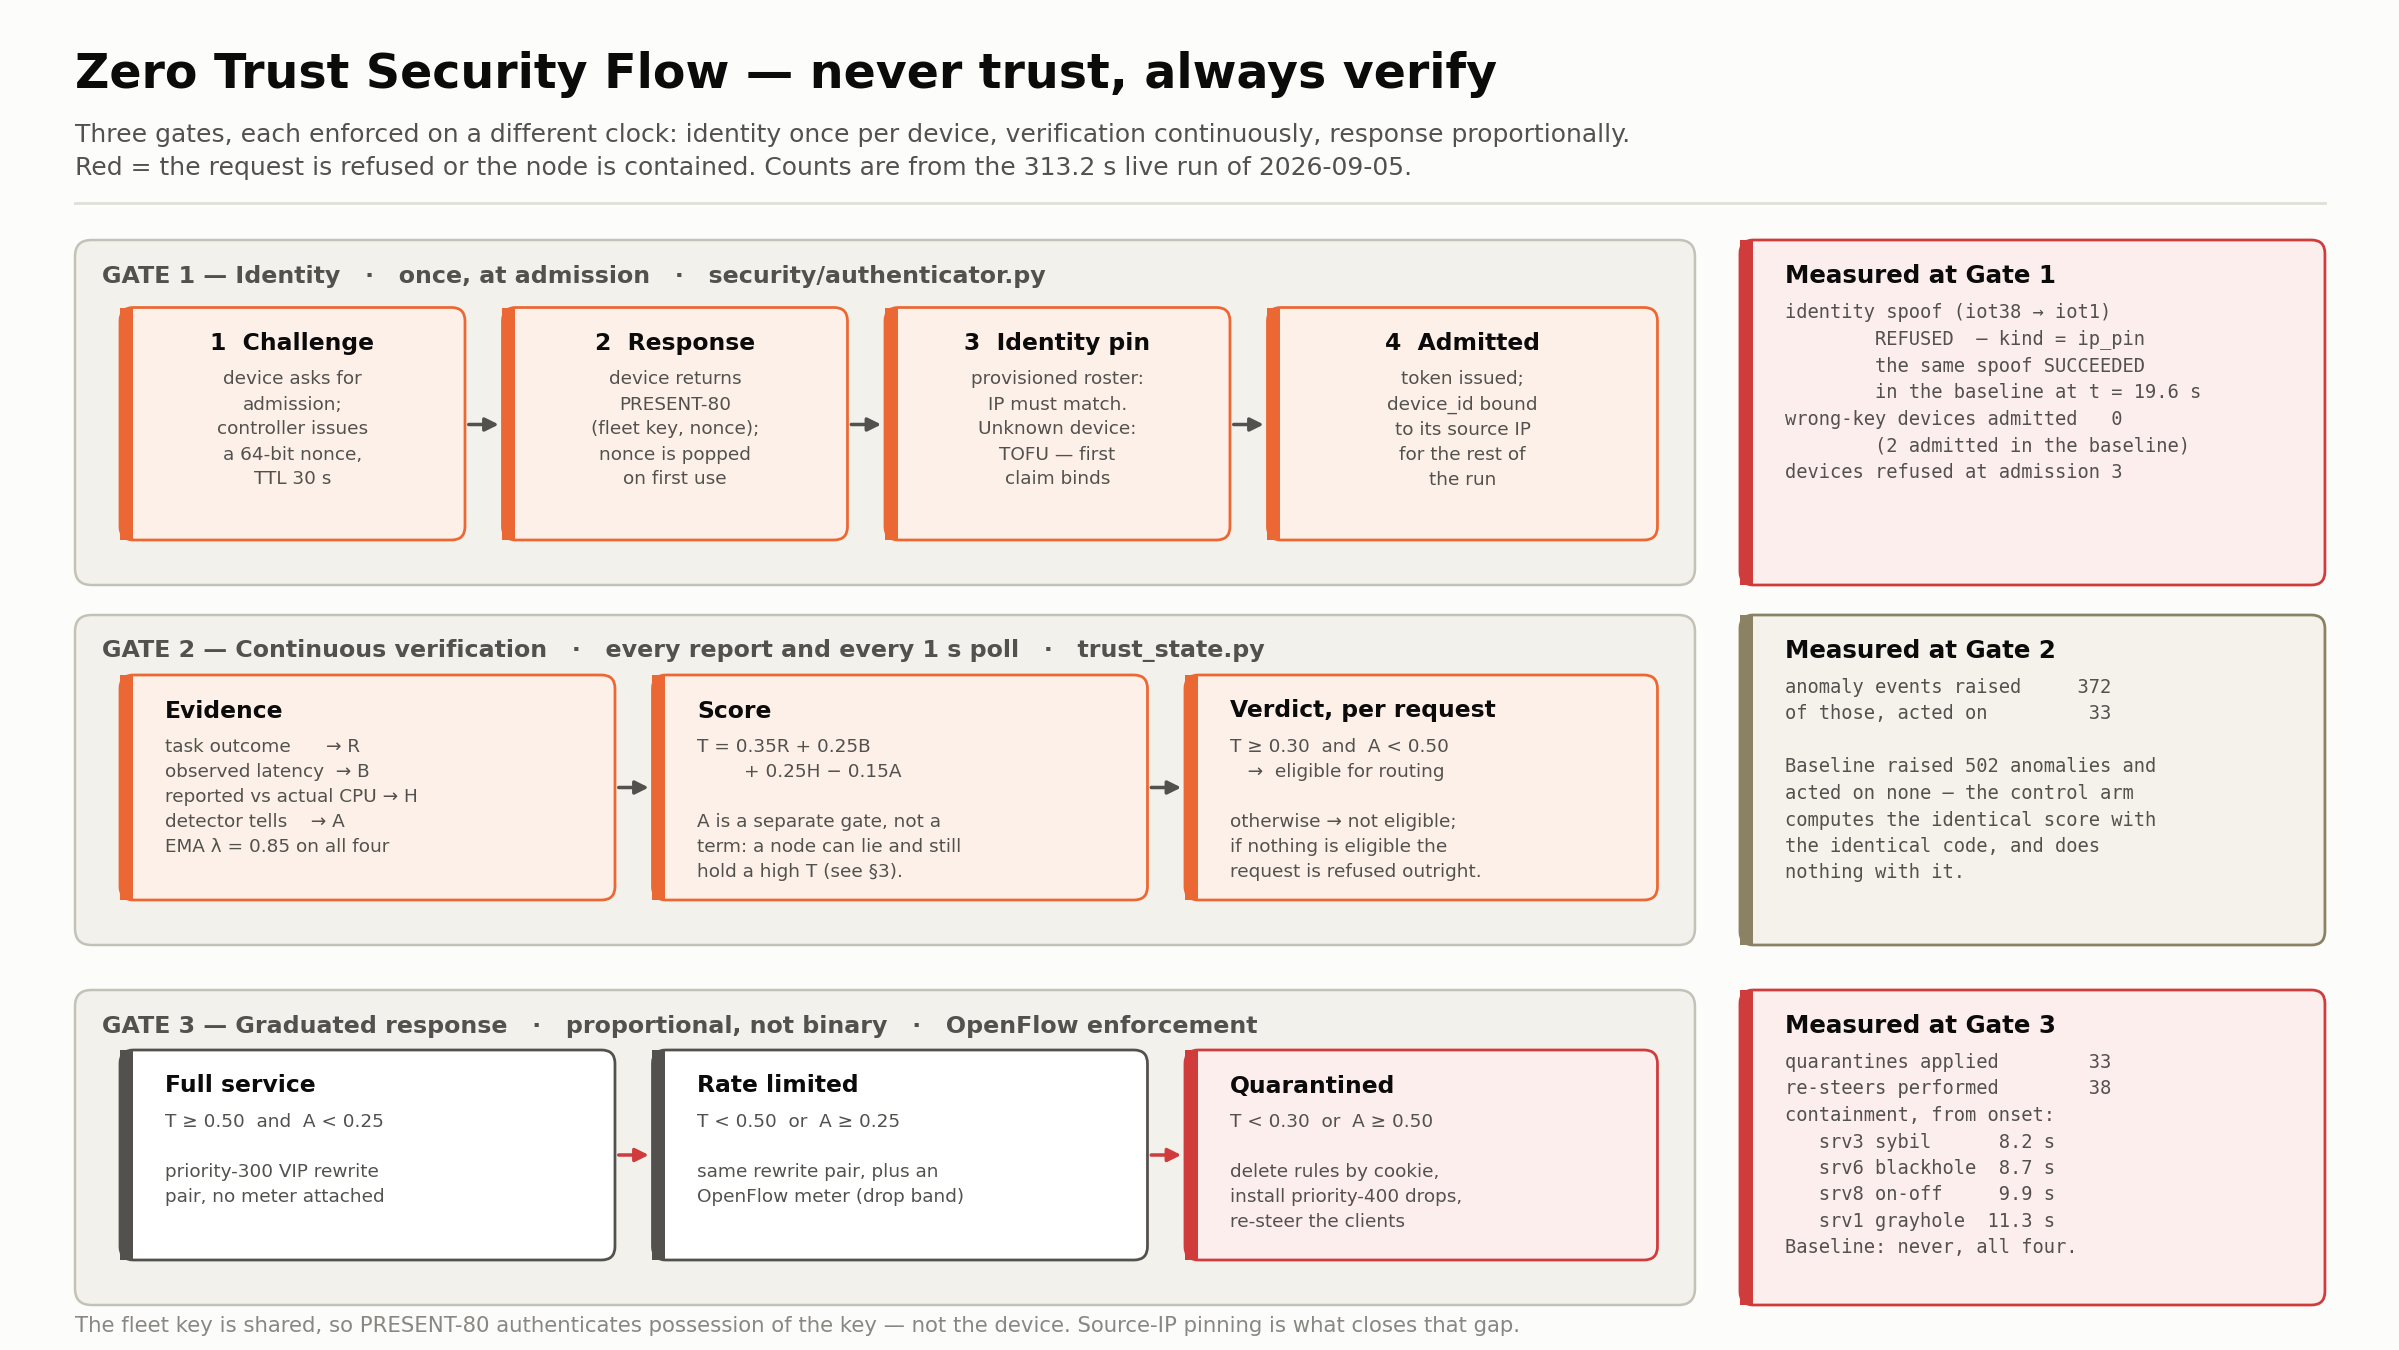
\includegraphics[width=\columnwidth]{fig6_zero_trust_flow.png}
\caption{The two decision rails. Trust \emph{ranks} eligible nodes; the anomaly
gate \emph{excludes} them, and exclusion is applied before ranking rather than
as a score penalty. The disjunction at the bottom is what the \armscore{} arm
ablates: $\Tscore < \theta$ \textbf{or} $\Agate \ge g$ becomes
$\Tscore < \theta$ alone.}
\label{fig:rails}
\end{figure}

The controller is a single OpenFlow~1.3~\cite{mckeown2008openflow}
application; the trust engine, the authenticator and the ledger are in-process
libraries. A client never addresses
a server: it connects to a virtual IP and the controller rewrites destination
MAC and IP in the data plane, so the routing decision is invisible to the
client and \emph{revocable} by the controller. One design rule runs through
every layer and is what makes the ablation cheap: the \emph{request} path
writes evidence into the trust state and the $1$\,Hz \emph{control} loop reads
decisions out of it, and the two never share a code path.

\subsection{Rail 1: the trust score}
Each completed task yields an update carrying task status, measured end-to-end
latency, the CPU load the node \emph{reported}, and the load the controller
\emph{observed}. Four features are extracted and smoothed with decay
$\lambda = 0.85$:
\begin{align*}
  r &= \begin{cases}1.0 & \text{success}\\ 0.3 & \text{timeout}\\ 0.0 & \text{failure}\end{cases}
  &
  b &= \max\!\left(0,\, 1 - \tfrac{\ell}{500\,\mathrm{ms}}\right)\\[2pt]
  h &= \max\!\left(0,\, 1 - \tfrac{\lvert c_{\mathrm{rep}} - c_{\mathrm{obs}}\rvert}{0.5}\right)
  &
  a &= \mathbb{1}[\text{anomaly raised}]
\end{align*}
and the composite is
\begin{equation}
  \Tscore \;=\; \alpha\bar{R} + \beta\bar{B} + \gamma\bar{H} - \delta\Agate,
  \label{eq:trust}
\end{equation}
with $\alpha{=}0.35$, $\beta{=}0.25$, $\gamma{=}0.25$, $\delta{=}0.15$, clipped
to $[0,1]$ and initialised at $0.5$. $\bar{R}$ is reputation from outcomes,
$\bar{B}$ behavioural consistency from latency, $\bar{H}$ resource honesty from
the claimed-versus-observed gap, and $\Agate$ a smoothed suspicion term.

\subsection{Rail 2: the anomaly gate}
The second rail is independent of Eq.~\ref{eq:trust} and its verdict is not a
weighted contribution to anything. A $1$\,Hz loop polls each node and runs four
detectors: a \textbf{latency tell} (a node claiming to be idle while answering
slower than a multiple of the \emph{fleet median}, requiring persistence across
three polls); a \textbf{timeout-rate tell} over a bounded window; a
\textbf{CPU-honesty check} comparing claimed busy time against the duty cycle
implied by the dispatches the controller saw complete, which \emph{abstains}
when the controller has too few completions rather than falling back to a fleet
comparison; and a \textbf{flood tell} keyed on the requesting client. Firings
are smoothed into $\Agate \in [0,1]$.

A node is quarantined when $\Tscore < \theta = 0.30$ \emph{or}
$\Agate \ge g = 0.50$ (Fig.~\ref{fig:rails}). The disjunction is the
architecture, and the second disjunct is what \S\ref{sec:res:ablation} removes.

\subsection{Selection, enforcement, and the exit from quarantine}
Exclusion is applied \emph{before} ranking. Among eligible nodes the controller
scores $w_1 \Tscore + w_2(1-\mathrm{cpu}) + w_3(1-\widehat{\ell})$ with
$w = (0.50, 0.30, 0.20)$ and selects by power-of-two-choices ($d{=}2$,
$\varepsilon = 0.05$). If every candidate is ineligible the request is denied ---
deny by default, never fall back to an untrusted node. Between ``full'' and
``quarantined'' sits a rate-limited band implemented with OpenFlow meters.

Once a rule is installed, matching packets are forwarded entirely in the data
plane and never return to the controller~\cite{mckeown2008openflow}, so all
controller-side observation in this paper is derived from $1$\,Hz flow-statistics
counters and endpoint reports rather than from per-packet inspection.

A decision becomes a flow-mod on a real switch: quarantine installs a
high-priority drop rule, deletes the node's serving rules by cookie, and
re-assigns in-flight dispatches. Quarantine naively implemented is an
\emph{absorbing state}, because isolating a node cuts exactly the traffic that
produces the outcomes $\bar{R}$ and $\bar{B}$ are built from. We close this with
\textbf{probation}, the half-open leg of a circuit
breaker~\cite{nygard2018releaseit}: a node quarantined on \emph{trust alone},
whose anomaly rail has fallen back below the gate, is offered one trial task
every $5$\,s. A node the gate has flagged is never probed.

\subsection{Naming the attack, admission, and audit}
A classifier turns detector signals into one discrete label per subject. It is
a pure function over an evidence \emph{window} --- not a single cycle --- because
two attack pairs are not separable from one cycle's signals: blackhole and
grayhole raise the same signal and differ in \emph{magnitude}; Sybil and on-off
raise the same signals and differ in \emph{intermittency}. The live controller
and the offline scorer call one implementation, so they cannot drift.

Devices authenticate by PRESENT-80 challenge--response with single-use nonces.
Because the key is fleet-wide the cipher authenticates \emph{possession of the
key}, not the \emph{device}; we close that with a source-IP pin against a
provisioned roster. A refusal returns HTTP~403 \emph{and} publishes an event,
so a denial is visible to the recording --- without which a spoof leaves no
trace and cannot appear in a confusion matrix. Trust updates are batched ten to
a block into a hash-chained ledger with a Merkle root per block; the dashboard
re-derives the chain in the browser rather than displaying the controller's own
validity flag, because a panel rendering that flag could never contradict it.

% ===========================================================================
\section{Why a Score Alone Cannot Isolate a Faithful Liar}
\label{sec:analysis}
% ===========================================================================

This section states what we expected the ablation to find, and why. It
concerns scores of the form of Eq.~\ref{eq:trust}: a convex combination of
service-derived features minus a bounded suspicion term.

\subsection{The faithful liar}
Define a \emph{faithful liar} as a node that misreports its resource state in
the direction that attracts traffic, but completes every task it accepts.
This adversary is the freeloading or traffic-harvesting node rather than the
saboteur, and it is the one an orchestrator scheduling on self-reported
telemetry is most exposed to. Against it the outcome-derived features are
pinned near their maxima: $\bar{R} \to 1$ because it never fails a task, and
$\bar{B} \to b$, its honest-latency value. Only $\bar{H}$ and $\Agate$ can move.

\begin{proposition}[Score floor]
\label{prop:floor}
Let $\Tscore = \alpha\bar{R} + \beta\bar{B} + \gamma\bar{H} - \delta\Agate$ with
$\alpha+\beta+\gamma+\delta = 1$, all weights non-negative and all smoothed
features in $[0,1]$. For a faithful liar with $\bar{R}=1$ and $\bar{B}=b$, and
for \emph{any} values of the remaining features,
$\Tscore \ge \alpha + \beta b - \delta$, attained at $\bar{H}=0$, $\Agate=1$.
\end{proposition}

\begin{proofsketch}
$\Tscore$ is non-decreasing in $\bar{H}$ and non-increasing in $\Agate$, so it
is minimised at $\bar{H}=0$, $\Agate=1$, giving $\alpha + \beta b - \delta$. No
further dishonesty reduces it, because the only negative term is scaled by
$\delta$ and $\Agate$ is already saturated.
\end{proofsketch}

The bound is elementary. What matters is what it is a bound \emph{on}: the
penalty available to any member of this score family is capped by
$\delta \le 1 - \alpha - \beta - \gamma$, \ie by whatever weight is left over
after the features that measure whether a node is doing its job. Isolating the
liar by score requires $\theta > \alpha + \beta b - \delta$; with our weights
and $b = 0.96$ at a $20$\,ms service latency that is $\theta > 0.44$, against a
shipped $\theta = 0.30$. Equivalently it requires $\delta > 0.29$, nearly
doubling the suspicion weight at the direct expense of the service terms. Both
moves make an honest node with one anomalous poll isolatable.

\subsection{The bound is valid and conservative}
\label{sec:analysis:conservative}
Proposition~\ref{prop:floor} predicts that the Sybil's score stays above
$\alpha + \beta b - \delta$. Computing that bound from each run's
\emph{measured} mean service latency for the Sybil node gives a predicted floor
of $0.302$ on average (range $0.278$--$0.328$) across the ten non-enforcing
runs. The measured minimum was $0.399$--$0.409$. The bound held in every run,
and it held loosely: the realised floor sat about $0.10$ above it.

The gap is instructive, and we prefer to explain it than to present the bound
as tighter than it is. The proposition's worst case assumes $\bar{H} \to 0$,
\ie that the honesty term is driven to zero. It is not. Over the Sybil's runs
the claimed-versus-observed load gap averaged $0.084$, so
$h = 1 - \text{gap}/0.5$ averaged $0.83$ and $\gamma\bar{H}$ contributed about
$+0.10$ to the score throughout. \emph{The term designed to punish lying barely
registered the lie}, because the normaliser assumes a gap the adversary never
has to open: under-reporting by a modest amount is enough to attract traffic
and leaves $\bar{H}$ high. The floor an adversary actually enjoys is therefore
higher than the analytic worst case, which strengthens rather than weakens the
conclusion.

What the proposition does not do is establish that the score fails in practice;
a bound of $0.30$ straddles $\theta = 0.30$. That is an empirical question, and
\S\ref{sec:res:ablation} answers it by experiment.

% ===========================================================================
\section{Evaluation Methodology}
\label{sec:method}
% ===========================================================================

\subsection{Testbed and workload}
One core switch and eight edge switches, all Open vSwitch speaking
OpenFlow~1.3 under Mininet~\cite{lantz2010mininet}, carrying eight edge servers
and forty IoT client processes on a four-core host. Servers perform \emph{real
bounded work} --- hash loops sized by a configured budget --- rather than
sleeping, which is what makes the telemetry measured rather than injected. Each
device reports every $2.0$\,s with a $15$\,ms task budget and a $4.0$\,s client
timeout: ${\sim}20$ requests/s from honest devices plus ${\sim}12$/s from the
flooding device. The rate is chosen so the \emph{control plane} --- the thing
under test --- is measured rather than starved.

Six attacks plus wrong-credential devices arm on a staggered schedule inside
every run: srv3 Sybil at $20$\,s, srv6 blackhole at $30$\,s, srv1 grayhole
($0.5$ drop rate) at $40$\,s, srv8 on-off ($20$\,s period, $0.5$ duty) at
$50$\,s, iot37 flood at $60$\,s, iot38 identity spoof at $15$\,s, and iot39--40
with wrong keys. Four servers and thirty-six devices are honest and must not be
flagged.

\subsection{The three arms}
\label{sec:method:arms}

\begin{table}[t]
\caption{The three arms. Each differs from the one above it by one mechanism.}
\label{tab:arms}
\centering\footnotesize
\begin{tabularx}{\columnwidth}{@{}lX@{}}
\toprule
\textbf{Arm} & \textbf{Enforcement}\\
\midrule
\armbase{}  & none. Static nearest-server routing; detectors run and publish,
              nothing acts on them.\\
\armscore{} & trust rail only. Quarantine, rate-limit and probation
              eligibility decided by $\Tscore < \theta$ alone.\\
\armfull{}  & both rails. $\Tscore < \theta$ \textbf{or} $\Agate \ge g$.\\
\bottomrule
\end{tabularx}
\end{table}

All three run the same topology, the same forty devices, the same six attacks
on the same schedule, launched by the same code, with trust computed by the
same estimators. \armbase{} is the no-enforcement control. \armscore{} is the
ablation that matters: it is the \emph{shipping controller} with one boolean
changed, and its configuration differs from \armfull{}'s in exactly two keys
--- the enforcement switch and the recording path --- which a test pins.

One subtlety decided the implementation. Setting the gate threshold to infinity
would have disabled the gate but \emph{also} removed the $\Agate$ term from
Eq.~\ref{eq:trust}, silently changing the score family and making the arms
incomparable. Instead the anomaly rail has a separate \emph{enforcement}
switch: $\Agate$ still enters the score in both arms, and only its ability to
\emph{act} is removed. Rows the \armbase{} arm cannot produce are reported as
\emph{not measured}, never as zero --- an absent mechanism is not a mechanism
that scored zero.

\subsection{Replication and statistical treatment}
\textbf{The unit of replication is the run.} Five runs per arm, fifteen live
runs in total, each ${\sim}320$\,s, executed in rotating arm order so machine
drift does not land on one arm. Per-task or per-route observations inside a run
are not independent replicates and are never pooled across runs.

Continuous metrics are reported as mean with a two-sided $95\%$ Student-$t$
interval over runs. Yes/no outcomes --- \emph{was this attacker isolated at
all}, \emph{did its score ever cross $\theta$} --- are reported as $k/n$ with a
Wilson interval~\cite{wilson1927}, never as a mean of 0/1s with a
$t$-interval, which is wrong at this $n$. Times are reported only over the runs
where the event happened, with $k/n$ alongside, because a run where it never
happened has no time to average and substituting the run length would invent
one.

With $n = 5$ per arm we report intervals and do not run significance tests
between arms on the service metrics; we describe two arms as separated only
when their intervals do not overlap, and say so explicitly when they do.

\subsection{The score rail is measured in every arm}
One measurement makes the ablation interpretable: for every attacker, in
\emph{all three arms including the ones that never act on it}, we record
whether and when $\Tscore$ first falls below $\theta$. This is the score rail's
verdict in isolation, observed even where it is not enforced, and it is the
direct test of \S\ref{sec:analysis}. We also record, at each first quarantine,
which rail could have caused it: $\Tscore < \theta$ only, $\Agate \ge g$ only,
or both. An arm that does not enforce the gate is always attributed to the
score, whatever $\Agate$ reads, because its gate cannot act.

\subsection{Simulation levels}
Two results in \S\ref{sec:res:sim} come from a seeded discrete-event
simulation driving the \emph{real} selector, trust calculator and both shipped
detectors: a comparison against four routing baselines over $600$ runs, and a
selector-scalability sweep to $N = 64$ that the four-core host cannot run live.
These are labelled as simulation wherever they appear and no live claim rests
on them.

% ===========================================================================
\section{Results}
\label{sec:results}
% ===========================================================================

All live figures come from fifteen runs archived under \texttt{data/runs/},
scored by one aggregator whose output ships with this draft.
\src{evidence/replicates/summary.txt}

\subsection{The ablation: what the score rail cannot reach}
\label{sec:res:ablation}

\begin{table}[t]
\caption{The central result. \emph{Score crossed $\theta$} is the trust rail's
own verdict, recorded in every arm including those that never act on it.
\emph{Quarantined} is what the arm actually did. Proportions carry Wilson
$95\%$ intervals; $\min \Tscore$ is the mean over runs of the lowest score
reached after onset.}
\label{tab:ablation}
\centering\footnotesize
\begin{tabular}{@{}llccc@{}}
\toprule
& & \armbase{} & \armscore{} & \armfull{}\\
\midrule
\multicolumn{5}{@{}l}{\textit{srv6 --- blackhole (fails every task)}}\\
& score crossed $\theta$ & 5/5 & 5/5 & 5/5\\
& quarantined            & ---  & \textbf{5/5} & \textbf{5/5}\\
& $\min \Tscore$         & 0.000 & 0.148 & 0.130\\
\midrule
\multicolumn{5}{@{}l}{\textit{srv1 --- grayhole (fails half its tasks)}}\\
& score crossed $\theta$ & 5/5 & 5/5 & 5/5\\
& quarantined            & ---  & \textbf{5/5} & \textbf{5/5}\\
& $\min \Tscore$         & 0.000 & 0.180 & 0.129\\
\midrule
\multicolumn{5}{@{}l}{\textit{srv3 --- Sybil (\textbf{never fails a task})}}\\
& score crossed $\theta$ & \textbf{0/5} & \textbf{0/5} & \textbf{0/5}\\
& quarantined            & ---  & \textbf{0/5} & \textbf{5/5}\\
& $\min \Tscore$         & 0.399 & 0.404 & 0.617\\
\midrule
\multicolumn{5}{@{}l}{\textit{srv8 --- on-off (\textbf{never fails a task})}}\\
& score crossed $\theta$ & \textbf{0/5} & \textbf{0/5} & \textbf{0/5}\\
& quarantined            & ---  & \textbf{0/5} & \textbf{5/5}\\
& $\min \Tscore$         & 0.411 & 0.399 & 0.548\\
\bottomrule
\end{tabular}

\vspace{3pt}
\begin{minipage}{\columnwidth}\scriptsize
$\theta = 0.30$. Wilson $95\%$ interval for 5/5 is $[57\%, 100\%]$ and for
0/5 is $[0\%, 43\%]$; the two do not overlap. ``---'' is \emph{not measured}:
\armbase{} has no quarantine mechanism.
\end{minipage}
\end{table}

Table~\ref{tab:ablation} is the paper's central result and it divides the four
server attacks into two groups along exactly the line
\S\ref{sec:analysis} predicts.

The two attackers that \textbf{fail tasks} --- the blackhole and the grayhole ---
drive $\bar{R}$ down, and their scores cross $\theta$ in every one of fifteen
runs. The score rail isolates them unaided: in \armscore{}, both are
quarantined 5/5.

The two attackers that \textbf{never fail a task} --- the Sybil and the on-off
attacker --- are a different matter. Their scores \textbf{never once cross
$\theta$}, in any arm, in any run: 0/15 each. Their minimum trust over a
$320$\,s run settles at $0.399$--$0.411$ in the arms that let them keep serving,
comfortably above the threshold and consistent with
\S\ref{sec:analysis:conservative}. With only the score rail enforced, neither
is \emph{ever} quarantined (0/5 each, Wilson $[0\%, 43\%]$). With the gate
enabled, both are quarantined in \emph{every} run (5/5 each, Wilson
$[57\%, 100\%]$).

This is the ablation's answer. The second rail is not a refinement of the
first. For half the server attacks in this threat model it is the only thing
that works at all.

\subsection{Which rail fired, and at what score}
\label{sec:res:rails}

\begin{table}[t]
\caption{At each attacker's first quarantine in \armfull{}: the rail that could
have caused it, and $\Tscore$ at that instant (mean over 5 runs,
$95\%$ $t$-interval).}
\label{tab:rails}
\centering\footnotesize
\begin{tabular}{@{}llcc@{}}
\toprule
\textbf{Node} & \textbf{Attack} & \textbf{Rail} & $\Tscore$ \textbf{at quarantine}\\
\midrule
srv6 & blackhole & score 4/5, both 1/5 & 0.130 [0.074, 0.185]\\
srv1 & grayhole  & both 3/5, gate 2/5  & 0.220 [0.066, 0.374]\\
srv3 & Sybil     & \textbf{gate 5/5}   & \textbf{0.710} [0.630, 0.791]\\
srv8 & on-off    & \textbf{gate 5/5}   & \textbf{0.709} [0.641, 0.777]\\
\bottomrule
\end{tabular}

\vspace{3pt}
\begin{minipage}{\columnwidth}\scriptsize
``both'' means $\Tscore < \theta$ \emph{and} $\Agate \ge g$ held at that
instant, so the score would have isolated the node unaided. Crediting the gate
in that case would overstate it.
\end{minipage}
\end{table}

Table~\ref{tab:rails} shows the same split from the enforcement side. The Sybil
and the on-off attacker are quarantined at a trust score of $0.71$ --- $2.4
\times$ the isolation threshold --- by a rail that is not part of the score.
The blackhole is isolated by the score in four of five runs, with the gate
merely concurring in the fifth. The grayhole sits between: both rails qualify
in three runs, the gate alone in two, which is the case where the gate is
simply faster.

We flag one measurement trap here because it changed a number in this table.
Attributing the rail from ``was $\Agate \ge g$ at that instant'' is wrong in
the \armscore{} arm, where $\Agate$ still rises but cannot act: every grayhole
quarantine there carries $\Agate \approx 1.0$ next to $\Tscore < \theta$, and a
naive reading credits a gate that was switched off. Attribution therefore
consults the arm's enforcement setting, and reports ``both'' rather than
``gate'' when both conditions hold.

\subsection{Containment latency}
\label{sec:res:contain}

\begin{table}[t]
\caption{Seconds from attack onset to isolation. Median over 5 runs, with the
range. \armbase{} never contains anything.}
\label{tab:contain}
\centering\footnotesize
\begin{tabular}{@{}llcc@{}}
\toprule
\textbf{Node} & \textbf{Attack} & \armscore{} & \armfull{}\\
\midrule
srv6 & blackhole & 10.7 (9.8--12.0)  & 10.1 (9.3--11.7)\\
srv1 & grayhole  & 15.6 (12.1--22.6) & 15.5 (12.3--31.7)\\
srv3 & Sybil     & \textbf{never}    & \textbf{7.6} (5.9--10.2)\\
srv8 & on-off    & \textbf{never}    & \textbf{10.4} (9.8--37.5)\\
\bottomrule
\end{tabular}
\end{table}

Where both arms contain an attacker they contain it at the same speed: the
score rail is not slower, it is simply blind to two of the four. The gate is
also the \emph{fastest} single detector in the set --- it reaches the Sybil in a
median $7.6$\,s, faster than the score reaches either of the task-failing
attackers --- because a latency tell needs three consecutive polls whereas a
timeout rate needs enough dispatches to accumulate.

Detection and response are effectively simultaneous: over the twenty
node-run pairs in the \armfull{} arm the gap between a node's first anomaly
event and its first quarantine ranged from $3.5$ to $12.5$\,ms, so the
latencies above are detection latencies. \src{data/runs/treat/}

\subsection{Service, availability and fairness}
\label{sec:res:service}

\begin{table*}[t]
\caption{Service and containment across the three arms. Mean over 5 runs with a
two-sided $95\%$ Student-$t$ interval. Bold marks an arm whose interval does
not overlap either of the others; where intervals overlap we draw no
conclusion. ``---'' is \emph{not measured}.}
\label{tab:service}
\centering\footnotesize
\begin{tabular}{@{}lccc l@{}}
\toprule
\textbf{Metric} & \armbase{} & \armscore{} & \armfull{} & \textbf{Reading}\\
\midrule
Packet delivery ratio        & 94.35\,\% [94.15, 94.55] & 99.40\,\% [99.29, 99.52] & 99.25\,\% [99.06, 99.44] & enforcement helps; rail choice does not\\
Tasks lost to timeout        & 377.8 [375.0, 380.6]     & 35.4 [26.8, 44.0]        & 43.2 [31.0, 55.4]        & enforcement helps; rail choice does not\\
Throughput (task/s)          & 20.15 [19.44, 20.86]     & 19.53 [19.23, 19.84]     & 19.72 [19.12, 20.31]     & all three overlap\\
Mean task latency            & 87.4\,ms [80.0, 94.7]    & 98.3\,ms [93.7, 103.0]   & 91.6\,ms [86.8, 96.5]    & all three overlap\\
$p95$ task latency           & 317.8\,ms [288.2, 347.3] & 175.6\,ms [161.1, 190.2] & \textbf{137.2\,ms} [128.5, 145.9] & the gate halves the tail again\\
Honest per-device availability& 85.72\,\% [85.63, 85.82] & 99.29\,\% [99.15, 99.43] & 99.13\,\% [98.92, 99.34] & enforcement helps; rail choice does not\\
Honest devices served $<50\%$ & 5.0 [5.0, 5.0]          & 0.0 [0.0, 0.0]           & 0.0 [0.0, 0.0]           & enforcement helps; rail choice does not\\
Jain fairness, honest servers & 0.676 [0.643, 0.709]    & 0.996 [0.994, 0.998]     & 0.996 [0.991, 1.000]     & enforcement helps; rail choice does not\\
Routes reaching attackers     & 29.84\,\% [28.63, 31.05] & 17.37\,\% [16.74, 18.00] & \textbf{11.63\,\%} [10.84, 12.42] & \textbf{the gate's main service effect}\\
Mean attacker time isolated   & ---                      & 41.38\,\% [40.21, 42.55] & \textbf{67.13\,\%} [64.28, 69.97] & \textbf{the gate's main effect}\\
\midrule
Honest servers ever quarantined & 0.0 & 0.0 & 0.0 & no false isolation in any arm\\
Honest subjects mislabelled     & 0.0 & 0.0 & 0.0 & no false accusation in any arm\\
Attackers quarantined pre-onset & 0.0 & 0.0 & 0.0 & no containment credit is spurious\\
\bottomrule
\end{tabular}
\end{table*}

Table~\ref{tab:service} separates three questions that a single-baseline
comparison conflates.

\textbf{Does enforcement help?} Unambiguously. Against the no-enforcement
control, either acting arm raises delivery ratio by about five points, cuts
timeouts by an order of magnitude, lifts honest per-device availability by
about thirteen points, removes all five starved devices, and lifts fairness
across honest servers from $0.68$ to $0.996$. Every one of those intervals is
disjoint from the control's.

\textbf{Does the \emph{choice of rail} help those service metrics?} No, and
this is the result a single-baseline design would have missed. \armscore{} and
\armfull{} overlap on delivery ratio, timeouts, throughput, mean latency,
honest availability and fairness. On the evidence here the gate buys no
service improvement over the score rail alone.

\textbf{What does the gate buy?} Containment. The share of traffic reaching
attacker nodes falls from $17.37\%$ to $11.63\%$ and mean attacker isolation
time rises from $41\%$ to $67\%$, both with disjoint intervals --- because two
of the four attackers are never isolated at all without it. The tail follows:
$p95$ latency falls from $176$\,ms to $137$\,ms, also disjoint. A faithful liar
degrades the service it accepts without ever failing a task, so removing it
from the rotation shows up in the tail rather than in the delivery ratio.

Two corrections to our own earlier reporting belong here. First, we previously
reported a mean-latency \emph{cost} for enforcement from a single run pair;
across replicates the three arms' mean-latency intervals all overlap and we
withdraw the claim. Second, we previously reported a throughput cost; those
intervals overlap too.

\paragraph*{Fairness needs two populations}
Jain's index over the \emph{whole} roster barely separates the arms
($0.605$/$0.681$/$0.622$) and read alone would say the load balancer made no
difference. Both extremes are uneven for opposite reasons: the control arm
because the flooding device is statically bound to one server that nothing can
move it off, the acting arms because they deliberately starve attackers.
\emph{Starving an attacker is correct behaviour and must not be scored as
unfairness.} Over the four honest servers, where the metric means what it is
for, the arms separate hard. We report both populations plus the attacker
share, and recommend the same for any trust-aware balancer evaluation.

\subsection{Detection quality}
\label{sec:res:detect}
Scoring all 48 subjects --- eight attackers and forty honest --- against ground
truth, over five runs per arm: overall accuracy is $91.67\%$ in \armbase{},
$97.92\%$ in \armscore{} and $97.50\%$ [$96.34$, $98.66$] in \armfull{}. Every
arm places $0/40$ honest subjects in an attack class, in every run. The acting
arms name $8/8$ attacks in the right \emph{family}; the control arm manages
$4/8$, because two of its attackers are never contained and two never register
on the rail that would name them.

Exact labels run $7.00$ in \armscore{} and $6.80$ [$6.24$, $7.36$] in
\armfull{}; the intervals overlap. The recurring miss is the blackhole labelled
\emph{grayhole} --- the right family, one step too mild --- because once it is
quarantined at ${\sim}10$\,s it receives almost no traffic and the timeout-rate
tell never accumulates a measured rate.

The zero false-positive rate on forty honest subjects across fifteen runs is
the number we would most want a reviewer to check, because it is what an
over-eager detector buys its recall with. ``No attack'' is scored as a real
class precisely so it cannot be hidden.

\subsection{Non-functional requirements}
\label{sec:res:nfr}
Over the five \armfull{} runs: routing decision (packet-in $\to$ flow-mod) mean
$0.54$--$0.55$\,ms, $p95$ $0.71$--$0.73$\,ms, max $4.4$--$8.6$\,ms, against a
$<200$\,ms requirement; isolation re-dispatch mean $12.9$--$23.5$\,ms, max
$32.8$\,ms, against $<3000$\,ms; ledger overhead $0.045$--$0.052\%$ of
end-to-end task latency over $625$--$661$ blocks, against $<15\%$.
\src{evidence/nfr\_replicates.txt}

Two readings matter more than the verdicts. The re-dispatch is three orders of
magnitude inside its bound, but the isolation time an operator experiences is
dominated by \emph{detection}, which is bounded below by the $1$\,s poll and
the three-poll persistence requirement. Tightening it means polling faster or
shortening persistence, and persistence is exactly what keeps healthy nodes out
of quarantine on a jitter blip. And tamper-evidence at this batch size is
effectively free.

\textbf{Raft is implemented, unit-proven for safety and demonstrated live over
TCP with a leader kill --- and the controller still commits single-replica.} A
recorded $45$\,s failover (Fig.~\ref{fig:raft}) shows $850$ of $853$ commits
succeeding, failover in $0.21$\,s, and an outage of three refused attempts.
Every block of every live run in this paper carries term $0$ and a single
proposer. Three runtime blockers stand between the built component and the
wired one: nothing drives the election tick, a commit would block an OpenFlow
handler thread for up to the commit timeout, and the current flush path
discards a \texttt{None} return, which under Raft means losing trust updates on
every leadership change. We name them rather than imply the live runs are
consensus-backed.

\begin{figure}[t]
\centering
\includegraphics[width=\columnwidth]{raft_failover.png}
\caption{Recorded Raft failover on a standalone three-replica cluster under
continuous load: leader killed at $15$\,s, restarted at $30$\,s. The gaps are
deliberate --- a dead replica's missing samples are left as gaps rather than
bridged, because a bridged line would assert it held its term while down.}
\label{fig:raft}
\end{figure}

\subsection{Simulation: baselines and scale}
\label{sec:res:sim}
Two questions need more repetitions or more nodes than a live testbed provides.
Both drive the \emph{real} selector, trust calculator and detectors inside a
seeded simulation; neither is a live claim.

\paragraph*{Against four routing baselines}
Five strategies $\times$ four scenarios $\times$ thirty seeds $= 600$ runs,
paired on seed with common random numbers, tested with the Wilcoxon
signed-rank test~\cite{wilcoxon1945} and Holm--Bonferroni
correction~\cite{holm1979} within scenario. Fourteen of sixteen comparisons
favour the full system, all at $p_{\mathrm{adj}} = 7.45\times10^{-9}$ with
rank-biserial $r = +1.00$. Under attack, SLO violations fall $15.1$--$29.8\%$
against a \emph{no-trust ablation} that is the same selector with only the
trust term removed, and $61.8$--$68.8\%$ against least-connections.
\src{evidence/stats\_slo.txt}

We attach a caveat to those $p$-values that we think should be standard. All
thirty seeds won in every favouring comparison, so $7.45\times10^{-9}$ is the
\emph{smallest value the test can return} at this $n$; it reflects a
deterministic ordering, not a large sample. The effect sizes and medians carry
the result, not the $p$-value.

The two losses are honest and instructive: in the \emph{no-attack} scenario the
system is $10.7\%$ worse than round-robin and $4.8\%$ worse than random. The
cause is not the trust term but the staleness of the load signal every
load-reactive strategy reads~\cite{mitzenmacher2000old,dahlin2000stale}: a poll
sweep shows the load-blind strategies flat and every load-reading strategy
improving monotonically as the signal freshens, with the full system best on
the board at a $0.01$\,s poll.

\paragraph*{Selector scalability}
Sweeping $N = 4 \ldots 64$ at $60\%$ offered load, power-of-two-choices scales
linearly ($48 \to 762$ task/s, delivery $99.7$--$99.8\%$) while $\arg\max$
saturates at ${\sim}85$ task/s with delivery collapsing to $10.5\%$. Two
qualifications keep this honest: $\arg\max$ fails \emph{differently} at the two
ends of load --- starving 13 of 16 nodes at $10\%$ load, and at $60\%$ ending up
balanced \emph{and} broken as queues push load off the favoured nodes --- and
p2c is \textbf{not} a per-decision CPU win, since both strategies cost
$3$--$30\,\mu$s across the sweep because the selector ranks every eligible node
either way to produce the decision's explanation. We claim the p2c win in
fairness, delivery and delay, never in CPU. \src{evidence/scalability.csv}

\paragraph*{The capacity cliff}
Isolating a node removes its capacity. At $N = 4$ with two attackers, isolating
half the fleet leaves the honest half near saturation and the queueing wipes
out the SLO gain --- the system \emph{loses} its headline metric while still
delivering $32\times$ fewer outright failures. By $N = 6$ the cliff is gone.
\textbf{The defence needs enough spare capacity to absorb what it isolates},
which is a deployment constraint with a measured shape.
\src{evidence/capacity\_cliff/}

% ===========================================================================
\section{Discussion}
\label{sec:discussion}
% ===========================================================================

\subsection{Enforcement corrupts its own input signal}
\label{sec:disc:feedback}
Data-plane enforcement has a consequence a simulated quarantine does not:
installing a drop rule \emph{tears down the in-flight TCP connections} to that
node. The client waits out its own timeout on a dead socket while the
controller's dispatch record has already moved to the survivor that inherited
the flow. The resulting timeout is charged to a node that was never asked to do
the work.

Uncorrected this closes a positive feedback loop --- false attribution lowers an
honest node's score, which quarantines it, which re-dispatches onto fewer
nodes, which produces real timeouts, which feed the drop tell. The correction
carries \textbf{no tuned threshold}: an inherited dispatch is stamped as such
at re-assignment, and the report path skips trust attribution for it while
\emph{still publishing} the event, so availability and delivery ratio keep
counting the client's real loss and the abstention is re-derivable offline. A
proposal to instead excuse a re-steered outcome that arrived with ``too little
budget remaining'' was tested against the recordings and would have excused
zero of twenty-six cases: the median re-steered flow still had $2.86$ of its
$4.0$\,s remaining. It was a wrong-node problem, not a partial-budget problem.

Across the five \armfull{} runs the rule fires on $123$ of $32{,}107$ reports,
$0.38\%$ (range $0.28$--$0.48\%$). \src{data/runs/treat/} That is a small number
that decides whether honest nodes are quarantined, and no honest server was
quarantined in any of the fifteen runs. The general lesson we would carry to
any system enforcing a verdict in the data path: \emph{the enforcement action
is itself an input to the detector, and the coupling must be made explicit or
it will be discovered as a cascade.}

\subsection{A retraction: containment does not cost attribution}
\label{sec:disc:retract}
An earlier version of this work claimed a \emph{containment--attribution
tension}: that isolating an attacker faster starves the evidence needed to name
what it did, so defence quality and label precision trade against each other.
The claim rested on three runs that differed in many things at once.

Replication does not support it. Over the ten acting runs, containment (mean
attacker time isolated) spans $40.0\%$ to $69.3\%$ --- a $29$-point range --- while
exact labels are $7/8$ in nine runs and $6/8$ in one. The Spearman correlation
is $\rho = -0.52$ with $p = 0.12$ at $n = 10$. A trade predicts $\rho < 0$, and
the point estimate has that sign, but at this $n$ nothing short of a clearly
negative $\rho$ with $p < 0.05$ would support it. More tellingly, the
\emph{direction} of the near-constant label accuracy across a large containment
range is what one would expect if the effect were small or absent.
\textbf{We withdraw the claim.} \src{evidence/replicates/summary.txt}

We report this at length for two reasons. It was one of two headline findings
in the earlier draft, and a reader comparing versions deserves to know which
way the evidence moved. And the failure mode is worth naming: three runs that
differ in containment \emph{and} in run length \emph{and} in code version
support almost any story one looks for.

What survives is narrower and still true: the specific mechanism is real ---
once the blackhole is quarantined its timeout-rate tell stops accumulating, and
that is why it is labelled grayhole --- but the effect does not show up as a
measurable trade at this scale.

\subsection{What an ablation buys that a baseline does not}
\label{sec:disc:ablation}
A comparison against an external baseline answers ``is our system better than
theirs?'' An ablation answers ``which of our parts is doing the work?'', and
only the second question has an actionable answer. Here it produced three
findings a baseline comparison would have missed: that the gate is
\emph{necessary} for half the attacks rather than merely helpful; that it
contributes \emph{nothing} to the service metrics a paper would naturally lead
with; and that the score rail, far from being slow, is simply blind --- it
contains what it can see at the same speed the gate does.

The ablation was cheap only because of the architectural rule in
\S\ref{sec:arch}: the request path writes evidence and the control loop reads
decisions through separate code paths, so enforcement can be removed without
touching the trust engine. We would recommend that separation to anyone
building a system of this shape, for the evaluation it makes possible as much
as for the design.

One implementation detail carried the validity of the whole comparison, and it
is the kind of thing that is easy to get silently wrong. Disabling the gate by
raising its threshold to infinity would also have removed $\Agate$ from
Eq.~\ref{eq:trust}, changing the score itself and making the arms measure
different quantities. Separating \emph{computing} $\Agate$ from \emph{acting}
on it is what keeps the ablation an ablation.

% ===========================================================================
\section{Threats to Validity}
\label{sec:validity}
% ===========================================================================

\paragraph*{Internal}
Five runs per arm is enough for between-run intervals and not enough for
distributional claims; we report intervals and decline significance tests
between arms on service metrics. Runs were executed in rotating arm order on
one otherwise-idle host, which controls for monotone drift but not for a
change that coincides with one arm's slots. The three arms share a codebase,
so a defect in the shared path would move all three together --- the ablation
is protected against confounds \emph{between} arms, not against a common-mode
error.

\paragraph*{Construct}
The central measurement --- ``did the score ever cross $\theta$'' --- is
threshold-relative, so it inherits our choice of $\theta = 0.30$. A
substantially higher $\theta$ would catch the Sybil and, per
\S\ref{sec:analysis}, would also put honest nodes at risk; we did not sweep
$\theta$ live and that is the most direct attack on this result. Isolation
stands in for the wireless-sensor notion of ``node death'' in our availability
metric because no energy model exists here and inventing one for mains-powered
servers would be a fabricated number; readers comparing against WSN lifetime
literature should treat the metric as redefined, not transferred.

\paragraph*{External}
An emulated network~\cite{lantz2010mininet} on a four-core host, not a field
deployment. Scalability beyond eight servers is simulation driving the real
selector and supports a claim about the \emph{selection rule}, not a capacity
figure for real machines. The Raft measurements are three OS processes over
loopback TCP with real process kills: the code, sockets and process boundaries
are real; only hardware separation is not. One workload shape, Poisson-like at
a fraction of farm capacity; bursty and heavy-tailed workloads are untested.

\paragraph*{Conclusion}
The simulation $p$-values are the smallest the test can return at $n = 30$ and
should be read as a deterministic ordering, not a large sample
(\S\ref{sec:res:sim}). The live results carry intervals rather than $p$-values
by design. Where arms overlap we say so rather than describing the point
estimates.

\paragraph*{Adversary}
The attacker model is \textbf{fixed and non-adaptive}. An adversary that
observes its own detection and modulates --- keeping the claimed-versus-observed
gap just under the honesty normaliser, or timing an on-off period against the
EMA window --- would evade the tells we implement. Our claim is bounded to the
seven behaviours in \S\ref{sec:threat}. Notably,
\S\ref{sec:analysis:conservative} shows the honesty term already barely
registers a \emph{non}-adaptive liar, so the margin an adaptive one would need
is small.

% ===========================================================================
\section{Limitations and Future Work}
\label{sec:limits}
% ===========================================================================

\begin{enumerate}[leftmargin=1.2em,itemsep=2pt,topsep=2pt]
\item \textbf{No live $\theta$ sweep.} The ablation shows the gate is necessary
  at the shipped threshold. It does not show no threshold would do, and
  \S\ref{sec:analysis} argues rather than measures that raising $\theta$ costs
  honest nodes. Sweeping $\theta$ live across the three arms is the single most
  valuable next experiment.
\item \textbf{DDoS response is detection-only.} Flooding is detected,
  attributed to the client and classified, but not throttled; that needs a
  per-client-IP OpenFlow path, and the present machinery is per-edge-node.
\item \textbf{Raft is not wired into the controller}
  (\S\ref{sec:res:nfr}); the three blockers are named and each is a real change.
\item \textbf{Five runs per arm}, one host, one topology size.
\item \textbf{Hand-set weights.} An online bandit explores a fixed arm set.
  Whether learned weights beat hand-tuned ones is well-posed in our harness and
  we have not answered it.
\item \textbf{The controller is a trusted single point}, in tension with the
  doctrine the system implements. Full control-plane distribution is the honest
  long-term item.
\item \textbf{PRESENT-80 is an architecture demonstration}, not a security
  claim.
\end{enumerate}

The most valuable next adversary is an \emph{adaptive} one: a node that watches
its own anomaly level and modulates to stay beneath the gate.
\S\ref{sec:analysis} says a score cannot catch a faithful liar; the open
question this work leaves is how much evidence a gate needs before an adversary
can starve it.

% ===========================================================================
\section{Reproducibility}
\label{sec:repro}
% ===========================================================================
Every number carries the artifact it was read from. The offline scorers read
the same append-only recordings the live dashboard streams, and none needs the
controller stack installed. Fifteen run recordings are archived under
\texttt{data/runs/<arm>/}; one aggregator produces every live figure in
\S\ref{sec:results}. On the machine used for this draft the test suite reports
$832$ passing and $11$ skipped, with no failures. Commands, with \texttt{EV} for \texttt{evaluation}:

\begin{table}[H]
\centering\footnotesize
\begin{tabularx}{\columnwidth}{@{}lX@{}}
\toprule
\textbf{Result} & \textbf{Command} (prefix \texttt{python3 -m})\\
\midrule
Tables \ref{tab:ablation}--\ref{tab:service} & \texttt{EV.replicates data/runs}\\
\S\ref{sec:res:nfr} & \texttt{EV.nfr\_report data/runs/treat/rNN.jsonl}\\
\S\ref{sec:res:sim} baselines & \texttt{EV.baseline --runs 30 --csv r.csv}\\
 & \texttt{EV.stats r.csv}\\
\S\ref{sec:res:sim} scale & \texttt{EV.scalability\_sweep --ns 4,8,16,32,64}\\
The live runs themselves & \texttt{sudo tools/run\_replicates.sh}\\
\bottomrule
\end{tabularx}
\end{table}

Live runs require root, Open vSwitch and Mininet, and overwrite the active
recording at start-up; the runner archives each run before the next begins.
\emph{A recording that is not archived the moment a run finishes cannot be
re-scored}, a discipline this project learned by losing one.

% ===========================================================================
\section{Conclusion}
% ===========================================================================
Zero Trust requires continuous verification and grants no standing trust.
Applied to the serving infrastructure of an edge network, that demand has a
consequence a trust \emph{score} cannot satisfy on its own. We removed the
second decision rail from a working Zero-Trust SDN load balancer and ran it
live: the two attackers that never fail a task were never isolated, in any of
five runs, while their trust scores sat around $0.40$ against a $0.30$
threshold --- and never crossed it in any of fifteen runs across all three arms.
Restoring the gate isolated both in every run, at trust scores of $0.71$. The
two attackers that do fail tasks were isolated by the score alone, at the same
speed, in every run. The score rail is not slow; for half of this threat model
it is blind.

We report equally that the gate bought no measurable improvement in delivery
ratio, throughput, mean latency, honest availability or fairness over the score
rail alone --- it bought containment and the latency tail --- and that a
containment-versus-attribution trade we previously claimed does not survive
replication, and is withdrawn.

The broader methodological point is that the ablation, not the baseline
comparison, is what produced every one of those findings. It was available only
because enforcement could be removed without touching the trust engine, and
only because disabling the gate's \emph{action} was kept separate from removing
its \emph{term} from the score. Both are cheap design decisions that a system
of this shape should make early, for the evaluation they make possible as much
as for the architecture.

% ===========================================================================
\section*{Data Availability}
% ===========================================================================
The fifteen live recordings, the aggregator output, and the simulation CSVs
behind every table are archived with the project repository under
\texttt{data/runs/}, \texttt{data/replicates/} and
\texttt{paper-draft/evidence/}. Recordings are JSONL event streams of
${\sim}130$\,MB each. \textsc{TODO before submission:} deposit at a persistent
archive and cite the DOI here.

\section*{Ethics}
No human subjects, no personal data, and no third-party network were involved.
All attacks were executed against an emulated network on a single host under
the authors' control. No institutional review was required.

\section*{Author Contributions (CRediT)}
\textsc{TODO before submission: confirm per-author roles.} The intended
statement is: \emph{Conceptualization, Methodology} --- all authors;
\emph{Software, Investigation, Data curation} --- all authors;
\emph{Formal analysis, Visualization, Writing --- original draft} --- all
authors; \emph{Supervision} --- R.~N.

\section*{Conflicts of Interest}
The authors declare no competing interests.

\section*{Funding}
This work received no external funding.

\section*{Acknowledgements}
We thank our faculty guide for continued supervision. The substitution of the
maintained Ryu fork for the framework originally specified was an
environment-driven engineering decision documented in the project repository.

\bibliographystyle{unsrt}
\bibliography{references}

\end{document}
